% ╔═══════════════════════════════════════════════════════════════════════════╗
% ║                     UNIVERSAL ACADEMIC REPORT TEMPLATE                    ║
% ║                           BRUFACE • ULB • UMONS                           ║
% ╚═══════════════════════════════════════════════════════════════════════════╝
%
% Author: Maximilien Zarioh (2025)
% ═════════════════════════════════════════════════════════════════════════════
%                              SCHOOL SELECTION
% ═════════════════════════════════════════════════════════════════════════════

\newcommand{\school}{BRUFACE}  % <<< BRUFACE or ULB or UMONS

% ═════════════════════════════════════════════════════════════════════════════
%                             DOCUMENT VARIABLES
% ═════════════════════════════════════════════════════════════════════════════

% Course Information
\newcommand{\coursecode}{MECA-H411}
\newcommand{\coursetitle}{Structural Analysis and Finite Elements}

% Document Title
\newcommand{\doctitle}{Motorcycle Suspension Springs Analysis}
\newcommand{\docsubtitle}{Laboratory Report}

% Authors (use \\ for multiple authors)
\newcommand{\docauthors}{%
	Ibrahim El Mankouri \\
	Ibrahima Sow \\
	Maximilien Zarioh%
}

% Supervisor(s) (use \\ for multiple supervisors)
\newcommand{\docsupervisors}{%
	Prof. Peter Berke \\
	Louis Remes \\
	Noémi Mertens%
}

% ═════════════════════════════════════════════════════════════════════════════
%                ⚠️ DO NOT MODIFY ANYTHING BELOW THIS LINE
% ═════════════════════════════════════════════════════════════════════════════

\documentclass[a4paper,12pt]{article}

% ─────────────────────────────────────────────────────────────────────────────
%                          CONDITIONAL DEFINITIONS
% ─────────────────────────────────────────────────────────────────────────────

\usepackage{ifthen}
\usepackage{etoolbox}

% Create boolean flags for each school
\newbool{isBRUFACE}
\newbool{isULB}
\newbool{isUMONS}
\newbool{isEnglish}
\newbool{hasSceau}

% Set flags based on school selection
\ifthenelse{\equal{\school}{BRUFACE}}{%
	\booltrue{isBRUFACE}
	\booltrue{isEnglish}
	\booltrue{hasSceau}
}{}

\ifthenelse{\equal{\school}{ULB}}{%
	\booltrue{isULB}
	\booltrue{isEnglish}
	\booltrue{hasSceau}
}{}

\ifthenelse{\equal{\school}{UMONS}}{%
	\booltrue{isUMONS}
	\boolfalse{isEnglish}
	\boolfalse{hasSceau}
}{}

% ─────────────────────────────────────────────────────────────────────────────
%                             LANGUAGE SETTINGS
% ─────────────────────────────────────────────────────────────────────────────

\ifbool{isEnglish}{%
	\usepackage[english]{babel}
}{%
	\usepackage[french]{babel}
}

\usepackage[utf8]{inputenc}
\usepackage[T1]{fontenc}
\usepackage{csquotes}

% ─────────────────────────────────────────────────────────────────────────────
%                             BIBLIOGRAPHY SETUP
% ─────────────────────────────────────────────────────────────────────────────

\usepackage[backend=biber, style=ieee]{biblatex}
\addbibresource{data/references.bib}

% ─────────────────────────────────────────────────────────────────────────────
%                                PACKAGES
% ─────────────────────────────────────────────────────────────────────────────

% Layout
\usepackage{geometry}
\geometry{margin=2cm}

% Line spacing
\usepackage{setspace}
\onehalfspacing

% Graphics & Colors
\usepackage{graphicx}
\usepackage{xcolor}
\usepackage[pages=some]{background}
\usepackage{tcolorbox}

% Typography - Times New Roman equivalent
\usepackage{mathptmx}  % Times font for text and math
\usepackage{textcomp}

% Math
\usepackage{amsmath, amssymb}

% Tables & Figures
\usepackage{booktabs}
\usepackage{array, tabularx, float, makecell, ragged2e}
\usepackage{subcaption}
\usepackage{caption}

% Lists
\usepackage{enumitem}

% Code Listings
\usepackage{listings}

% Hyperlinks
\usepackage{hyperref}
\hypersetup{
	colorlinks=true,
	linkcolor=black,
	filecolor=magenta,
	urlcolor=blue,
	citecolor=blue,
	pdftitle={\doctitle},
	pdfauthor={Maximilien Zarioh},
}

% Ensure numbering is active by default (Section down to Subsubsection)
\setcounter{secnumdepth}{3}

% PGFPlots for graphs
\usepackage{pgfplots}
\pgfplotsset{compat=1.18}

% Calendar (for date calculations)
\usepackage{pgfcalendar}

% ─────────────────────────────────────────────────────────────────────────────
%                             CUSTOM SETTINGS
% ─────────────────────────────────────────────────────────────────────────────

% Table settings
\renewcommand{\tabularxcolumn}[1]{m{#1}}
\newcolumntype{C}{>{\Centering\arraybackslash}X}

% Code listing style
\definecolor{bg}{rgb}{0.95,0.95,0.95}
\lstdefinestyle{custom}{
	backgroundcolor=\color{gray!10},
	basicstyle=\ttfamily\footnotesize,
	breaklines=true,
	frame=single,
	numbers=left,
	numberstyle=\tiny,
	keywordstyle=\color{blue},
	commentstyle=\color{gray!70},
	stringstyle=\color{orange},
	tabsize=2,
	captionpos=b
}
\lstset{style=custom}


% ─────────────────────────────────────────────────────────────────────────────
%                         ACADEMIC YEAR CALCULATION
% ─────────────────────────────────────────────────────────────────────────────

\newcommand{\academicyear}{%
	\ifnum\month<9
	\number\numexpr\year-1\relax--\number\year
	\else
	\number\year--\number\numexpr\year+1\relax
	\fi
}

% Language-dependent "Academic Year" label
\ifbool{isEnglish}{%
	\newcommand{\academicyearlabel}{Academic Year}
}{%
	\newcommand{\academicyearlabel}{Année académique}
}

% ─────────────────────────────────────────────────────────────────────────────
%                           BACKGROUND SCEAU SETUP
% ─────────────────────────────────────────────────────────────────────────────

\ifbool{hasSceau}{%
	\backgroundsetup{
		scale=1,
		color=black,
		opacity=0.05,
		angle=15,
		position={13cm,-23cm},
		contents={%
			\includegraphics[height=15cm,width=15cm,keepaspectratio]{data/logos/sceau_ulb.jpg}
		}%
	}
}{}

% ─────────────────────────────────────────────────────────────────────────────
%                          TITLE PAGE CONFIGURATION
% ─────────────────────────────────────────────────────────────────────────────

% School-specific logo paths
\ifbool{isBRUFACE}{%
	\newcommand{\logoconfig}{%
		\begin{minipage}[c]{0.3\textwidth}
			\raggedright
			\includegraphics[height=1.5cm]{data/logos/logo_ulb.png}
		\end{minipage}%
		\hfill
		\begin{minipage}[c]{0.3\textwidth}
			\centering
			\includegraphics[height=1.5cm]{data/logos/logo_bruface.png}
		\end{minipage}%
		\hfill
		\begin{minipage}[c]{0.3\textwidth}
			\raggedleft
			\includegraphics[height=1.5cm]{data/logos/logo_vub.png}
		\end{minipage}%
	}
	\newcommand{\schoolname}{Brussels Faculty of Engineering}
	\newcommand{\facultyname}{}
}{}

\ifbool{isULB}{%
	\newcommand{\logoconfig}{%
		\begin{minipage}[c]{0.48\textwidth}
			\raggedright
			\includegraphics[height=1.8cm]{data/logos/logo_ulb.png}
		\end{minipage}%
		\hfill
		\begin{minipage}[c]{0.48\textwidth}
			\raggedleft
			\includegraphics[height=1.8cm]{data/logos/logo_epb.png}
		\end{minipage}%
	}
	\newcommand{\schoolname}{Université Libre de Bruxelles}
	\newcommand{\facultyname}{École Polytechnique de Bruxelles}
}{}

\ifbool{isUMONS}{%
	\newcommand{\logoconfig}{%
		\begin{minipage}[c]{0.48\textwidth}
			\raggedright
			\includegraphics[height=1.8cm]{data/logos/logo_umons.png}
		\end{minipage}%
		\hfill
		\begin{minipage}[c]{0.48\textwidth}
			\raggedleft
			\includegraphics[height=1.8cm]{data/logos/logo_fpms.png}
		\end{minipage}%
	}
	\newcommand{\schoolname}{Université de Mons}
	\newcommand{\facultyname}{Faculté Polytechnique de Mons}
}{}

% Language-dependent labels
\ifbool{isEnglish}{%
	\newcommand{\authorlabel}{Written by}
	\newcommand{\supervisorlabel}{Supervised by}
	\newcommand{\bibliographytitle}{Bibliography}
	\newcommand{\bibarticles}{Journal Articles}
	\newcommand{\bibbooks}{Books}
	\newcommand{\bibbooklets}{Booklets}
	\newcommand{\bibinbook}{Book Chapters}
	\newcommand{\bibincollection}{Articles in a Collection}
	\newcommand{\bibinproceedings}{Conference Proceedings}
	\newcommand{\bibmanual}{Manuals}
	\newcommand{\bibmastersthesis}{Master's Theses}
	\newcommand{\bibphdthesis}{PhD Theses}
	\newcommand{\bibproceedings}{Conference Proceedings (Book of Proceedings)}
	\newcommand{\bibreport}{Reports}
	\newcommand{\bibunpublished}{Unpublished Manuscripts}
	\newcommand{\bibmisc}{Miscellaneous References}
	\newcommand{\bibonline}{Web Pages}
	\newcommand{\bibpatent}{Patents}
	\newcommand{\bibstandard}{Standards}
}{%
	\newcommand{\authorlabel}{Rédigé par}
	\newcommand{\supervisorlabel}{Sous la direction de}
	\newcommand{\bibliographytitle}{Bibliographie}
	\newcommand{\bibarticles}{Articles de revues}
	\newcommand{\bibbooks}{Livres}
	\newcommand{\bibbooklets}{Livrets}
	\newcommand{\bibinbook}{Chapitres de livres}
	\newcommand{\bibincollection}{Articles dans une collection}
	\newcommand{\bibinproceedings}{Actes de conférences}
	\newcommand{\bibmanual}{Manuels}
	\newcommand{\bibmastersthesis}{Mémoires de Master}
	\newcommand{\bibphdthesis}{Thèses de doctorat}
	\newcommand{\bibproceedings}{Actes de conférences (livre des actes)}
	\newcommand{\bibreport}{Rapports}
	\newcommand{\bibunpublished}{Manuscrits non publiés}
	\newcommand{\bibmisc}{Références diverses}
	\newcommand{\bibonline}{Pages Web}
	\newcommand{\bibpatent}{Brevets}
	\newcommand{\bibstandard}{Normes}
}

% ═════════════════════════════════════════════════════════════════════════════
%                             DOCUMENT BEGINS HERE
% ═════════════════════════════════════════════════════════════════════════════

\begin{document}
	
	% ─────────────────────────────────────────────────────────────────────────
	%                              TITLE PAGE
	% ─────────────────────────────────────────────────────────────────────────
	
	\begin{titlepage}
		\ifbool{hasSceau}{\BgThispage}{}
		
		\begin{center}
			% ─── LOGOS ───────────────────────────────────────────────────────
			\logoconfig
			\vspace{3cm}
			
			% ─── COURSE CODE ─────────────────────────────────────────────────
			{\Large\textsc{\coursecode}}
			\vspace{0.3cm}
			
			% ─── COURSE TITLE ────────────────────────────────────────────────
			{\LARGE\textbf{\coursetitle}}
			\vspace{1.5cm}
			
			% ─── DOCUMENT TITLE ──────────────────────────────────────────────
			\rule{\textwidth}{1.6pt}
			\vspace*{-\baselineskip}
			\vspace*{-11pt}
			\rule{\textwidth}{0.4pt}
			\vspace{0\baselineskip}
			
			{\Huge\bfseries\doctitle}
			
			\vspace{\baselineskip}
			{\Large\textit{\docsubtitle}}
			
			\vspace{0\baselineskip}
			\rule{\textwidth}{0.4pt}
			\vspace*{-\baselineskip}
			\vspace{-10pt}
			\rule{\textwidth}{1.6pt}
			\vspace{1.5cm}
			
			% ─── AUTHORS AND SUPERVISORS ─────────────────────────────────────
			\begin{minipage}[t]{0.45\textwidth}
				\begin{flushleft}
					\large
					\textbf{\authorlabel}\\[0.3cm]
					\docauthors
				\end{flushleft}
			\end{minipage}%
			\hfill
			\begin{minipage}[t]{0.45\textwidth}
				\begin{flushright}
					\large
					\textbf{\supervisorlabel}\\[0.3cm]
					\docsupervisors
				\end{flushright}
			\end{minipage}
			
			\vfill
			
			% ─── ACADEMIC YEAR ───────────────────────────────────────────────
			{\large\textsc{\academicyearlabel{} \academicyear}}
			
		\end{center}
	\end{titlepage}
	
	% ─────────────────────────────────────────────────────────────────────────
	%                          TABLE OF CONTENTS
	% ─────────────────────────────────────────────────────────────────────────
	
	\pagenumbering{gobble}
	\tableofcontents
	\newpage
	
	% ─────────────────────────────────────────────────────────────────────────
	%                               CONTENT
	% ─────────────────────────────────────────────────────────────────────────
	
	\pagenumbering{arabic}
	
	% Part I - Project Assignment
\section*{Introduction}
\addcontentsline{toc}{section}{Introduction}
\label{chap:introduction}

The objective of this project is to perform a structural analysis of a motorcycle suspension spring, specifically the rear spring of a Kawasaki ZR-7. This analysis applies the Finite Element Method (FEM) \cite{course_notes} to solve a practical engineering problem.

The project pursues four main goals, as outlined in the assignment description \cite{project_assignment}. First, we aim to understand the mathematical formulation of finite elements, focusing on the linear tetrahedral element (TETRA4). Second, the project requires gaining proficiency in Salome-Meca for pre-processing and post-processing tasks. Third, we must build a custom finite element code in Python that implements stiffness matrix assembly, boundary condition application, and stress computation. Finally, the project involves a critical analysis of the results to understand the limitations of the chosen element types and the assumptions made during modeling.

This report is divided into two parts. Part I describes the model setup for the Kawasaki ZR-7 spring, presents the numerical results compared with experimental data, and discusses the validity of our assumptions. Part II details the verification of our custom Python implementation through patch tests and convergence studies.

\section{Model setup}
\label{chap:model_setup}

This chapter details the numerical models developed for this study. We began with a preliminary convergence study on a plate with a hole to validate our mesh refinement strategy, before modeling the Kawasaki ZR-7 suspension springs. All geometries and meshes were generated using Salome-Meca.

\subsection{Preliminary study: plate with a hole}
\label{sec:plate_model}

To understand the influence of mesh density on solution accuracy, we first analyzed a classic stress concentration problem: a thin rectangular plate with a central circular hole subjected to uniform traction.

\subsubsection{Geometry and boundary conditions}
The plate has a length $L = 520$ mm, a half-height $h = 180$ mm (total height $H=360$ mm), and a thickness $t = 2$ mm. A central hole of radius $R = 3.2$ mm is located at the geometric center. The material is linear elastic steel with Young's modulus $E = 210$ GPa and Poisson's ratio $\nu = 0.3$.

The loading consists of a uniform surface traction $T_x = 81$ N/mm$^2$ applied to the left and right edges. Appropriate constraints were applied to prevent rigid body motion while allowing Poisson contraction.

\subsubsection{Mesh strategy}
Four tetrahedral meshes were generated with increasing density: "Coarse", "Moderate", "Fine", and "Very Fine". The refinement focused on the region around the hole where high stress gradients were expected.

\subsection{Kawasaki ZR-7 front spring}
\label{sec:front_spring_model}

The front suspension spring of the Kawasaki ZR-7 is a helical compression spring. Due to the high computational cost of meshing the full geometry, we investigated simplified models using reduced numbers of coils.

\subsubsection{Geometry and material}
The spring is defined by a free length $L_0 = 416$ mm, an outer diameter $D_{ext} = 34$ mm, a wire diameter $d = 4.7$ mm, and a total of $n = 26$ coils (with 24 active coils). The geometry was generated using a parametric Python script \cite{helix_salome}. The material properties are identical to those of the plate ($E=210$ GPa, $\nu=0.3$).

\subsubsection{Finite element models}
Three distinct geometric models were created to test the validity of simplifying the spring domain. A 1-coil model was used to simulate an infinite spring with periodic-like conditions. A 2-coil model helped introduce interactions between coils, while a 3-coil model provided a closer approximation to the boundary effects found in the actual component.

\subsubsection{Boundary conditions}
The simulation mimics a compression test. The bottom surface was fully fixed ($u_x = u_y = u_z = 0$), while an imposed vertical displacement $\delta_z = -1$ mm was applied to the top surface. Horizontal degrees of freedom at the top were fixed ($u_x = u_y = 0$) to simulate flat parallel plates. The spring stiffness $k$ was computed as the total reaction force in the Z-direction divided by the applied displacement ($k = F_z / \delta_z$). The results from these reduced models were extrapolated to the full 24-active-coil spring using series spring theory.

\subsection{Rear spring model}
\label{sec:rear_spring_model}

The rear spring is significantly stiffer and larger. Its dimensions ($D_{ext} = 80$ mm, $d=11$ mm, $L_0 = 195$ mm, $n=6$) were measured experimentally. A single geometric model representing a 3-coil section was used with boundary conditions identical to the front spring. Four mesh densities were tested to ensure convergence.
  % FE Model Setup
\section{Numerical results}
\label{chap:results}

This chapter presents the results of the Finite Element analyses. We evaluate the convergence behavior of our models and compare the computed stiffness values with experimental measurements.

\subsection{Plate with hole: stress convergence}
The maximum Von Mises stress at the hole edge was computed for four mesh densities. The results are summarized in Table \ref{tab:plate_results} and visualized in Figure \ref{fig:plate_convergence}.

The theoretical maximum stress, calculated using the analytical solution for an infinite plate with a hole ($K_t \approx 3$), is $\sigma_{max} = 236.56$ MPa. The "Very Fine" mesh yields a value of 233.48 MPa, which is within 1.3\% of the theoretical target, demonstrating excellent convergence.

\subsection{Front spring stiffness}
The stiffness $k$ of the front spring was calculated for the 1-coil, 2-coil, and 3-coil models across four mesh densities. The results were extrapolated to the full spring (26 coils total, 24 active) and are presented in Table \ref{tab:front_spring_results} and Figure \ref{fig:front_spring_convergence}.

Comparing the three geometric models in Table \ref{tab:front_spring_results}, we observe that adding coils progressively reduces the stiffness for a given mesh density (e.g., from 12.20 kN/m to 11.90 kN/m for the Coarse mesh). This confirms that boundary effects are better captured by the 3-coil model.

The experimental stiffness is $k_{exp} = 7.2$ kN/m. The 3-coil model with the "Very Fine" mesh performs best, predicting a stiffness of 7.73 kN/m. This overestimation is typical for TETRA4 elements, which tend to be overly stiff, but the value is reasonably close to reality.

\subsection{Rear spring stiffness}
For the rear spring (6 coils total, 4 active), the numerical results are shown in Table \ref{tab:rear_spring_results} and plotted in Figure \ref{fig:rear_spring_convergence}.

The experimental stiffness is $k_{exp} = 85.3$ kN/m. Interestingly, the "Fine" mesh result (85.16 kN/m) is incredibly close to the experimental value, while the more refined "Very Fine" mesh yields a lower stiffness (78.14 kN/m, $-8.4\%$ error). This counter-intuitive result suggests that the "Fine" mesh result was fortuitously accurate due to error cancellation, whereas the "Very Fine" model has converged to a numerical solution that differs from the experimental reality (likely due to geometric simplifications or boundary condition idealizations).
  % Numerical Results
\section{Discussion}
\label{chap:discussion}

\subsection{Element performance and shear locking}
Throughout this study, we utilized linear tetrahedral elements (TETRA4). It is well known in finite element theory \cite{tetra4_theory} that linear tetrahedra can exhibit "volumetric locking" or "shear locking," particularly in bending-dominated problems. This results in an artificially stiff response.

This behavior explains why our coarse meshes consistently overestimated the stiffness (or underestimated the displacement) for the springs. As the mesh was refined, the stiffness values decreased, converging towards a softer solution. For the front spring, the converged value (7.73 kN/m) remained slightly above the experimental value (7.2 kN/m), consistent with the stiff nature of TETRA4 elements.

\subsection{The "better" coarse mesh anomaly}
In the rear spring analysis, the "Fine" mesh seemingly produced a "better" result ($k \approx 85.16$ kN/m) than the "Very Fine" mesh ($k \approx 78.14$ kN/m), when compared to the experimental reference ($k_{exp} = 85.3$ kN/m).

The "Very Fine" mesh is numerically superior and provides a result closer to the exact solution of the \textit{mathematical model}. The fact that it drifts further from the \textit{experimental} value indicates that the mathematical model itself (geometry, boundary conditions, material properties) has discrepancies with physical reality. The "Fine" mesh result was merely a coincidence where discretization error cancelled out modeling error. We must trust the converged solution (78.14 kN/m) as the true prediction of our model, even if it is less accurate experimentally.

\subsection{Model limitations and improvements}
Several factors contribute to the discrepancy between our converged FEM results and experimental data. First, the use of linear tetrahedral elements introduces artificial stiffening, which could be mitigated by switching to quadratic tetrahedra (TETRA10) or hexahedral elements to improve accuracy for the same mesh density. Second, our boundary conditions assume a "flat plate" compression with fixed radial degrees of freedom ($u_x=u_y=0$), whereas in reality, the spring ends can slip or expand slightly, reducing the effective stiffness. Finally, the geometric simplification of modeling only a few coils ignores the complex contact mechanics at the spring ends (closed and ground ends), which significantly affects the number of active coils.

To address these limitations and improve the model fidelity, future work should prioritize employing high-order elements to eliminate shear locking. Additionally, modeling the full spring geometry, including ground ends and transition coils, would allow us to capture realistic boundary effects. Instead of relying on generic specifications, a 3D scan of the actual test specimens would also provide a direct validation of the geometric model.
  % Discussion
\section{Conclusion}
\label{chap:conclusion}

This project successfully demonstrated the complete finite element analysis workflow for a motorcycle suspension spring, from CAD geometry generation to the validation of a custom solver code.

\subsection{Summary of achievements}

We developed proficiency in the Salome-Meca platform by executing both a preliminary plate analysis and a complex spring study. Three successive spring models (1, 2, and 3 coils) were created with increasing mesh density, and the convergence study confirmed the mesh independence of the reaction force. By modeling a 3-coil section, we were able to approximate the full spring behavior while maintaining computational efficiency. The numerical stiffness was then compared against physical measurements, allowing us to attribute discrepancies to specific factors like element formulation and geometric simplifications. Finally, a rigorous suite of verification tests confirmed the correctness of our custom FEM implementation, validating our element formulation, assembly, and boundary condition algorithms.

\subsection{Key learnings}

A critical takeaway from this project is that element selection matters significantly; linear tetrahedra exhibit stiffness issues in bending-dominated problems, necessitating higher-order elements for accuracy. Furthermore, we reinforced the distinction between verification and validation: while patch tests ensure mathematical correctness, validation against experimental data is essential to assess physical accuracy. Most importantly, we observed that convergence is necessary but not sufficient, as a converged FEM solution only guarantees control over discretization error, not agreement with physical reality.
  % Conclusions
\section{Work distribution and transparency}
\label{chap:work_distribution}

\subsection{Work distribution}
The workload for this project was divided among the group members as follows:

\begin{description}[style=multiline, leftmargin=5cm, font=\bfseries]
    
    \item[Ibrahim El Mankouri]
    \begin{itemize}[leftmargin=*, label=$\cdot$, noitemsep]
        \item Salome-Meca modeling (front \& rear springs)
        \item Drafting spring modeling sections (sections \ref{sec:front_spring_model} \& \ref{sec:rear_spring_model})
        \item Analysis of numerical results (section \ref{chap:results})
    \end{itemize}

    \item[Ibrahima Sow]
    \begin{itemize}[leftmargin=*, label=$\cdot$, noitemsep]
        \item Preliminary study modeling (section \ref{sec:plate_model})
        \item Drafting of theoretical framework \& discussion (section \ref{chap:discussion})
        \item Drafting introduction
    \end{itemize}

    \item[Maximilien Zarioh]
    \begin{itemize}[leftmargin=*, label=$\cdot$, noitemsep]
        \item Python FE solver development
        \item Salome-to-Python integration
        \item Code verification \& validation (part II - section \ref{chap:verification})
        \item Final report structure \& \LaTeX\ formatting
    \end{itemize}
    
\end{description}

\subsection{Use of generative AI}
In accordance with the project guidelines regarding the responsible use of Artificial Intelligence, we declare the following:

Generative AI tools were employed exclusively to assist with the structure, clarity, and grammatical correctness of this report. Specifically:
\begin{itemize}
    \item AI was used to suggest improvements to sentence structure and vocabulary to ensure a professional academic tone.
    \item AI was used to assist with \LaTeX\ formatting issues.
    \item AI was used to write the \LaTeX\ code for the convergence graphs (Figures \ref{fig:plate_convergence}, \ref{fig:front_spring_convergence}, and \ref{fig:rear_spring_convergence}) based on our results.
\end{itemize}

No part of the Python code implementation was generated by AI. All algorithms, including the element stiffness matrix formulation, assembly procedures, and boundary condition applications, were written manually.  % Work distribution and AI usage
\section{References}
\label{chap:bibliography}


\printbibliography[heading=subbibliography, type=article, title={\bibarticles}]
\printbibliography[heading=subbibliography, type=book, title={\bibbooks}]
\printbibliography[heading=subbibliography, type=booklet, title={\bibbooklets}]
\printbibliography[heading=subbibliography, type=inbook, title={\bibinbook}]
\printbibliography[heading=subbibliography, type=incollection, title={\bibincollection}]
\printbibliography[heading=subbibliography, type=inproceedings, title={\bibinproceedings}]
\printbibliography[heading=subbibliography, type=manual, title={\bibmanual}]
\printbibliography[heading=subbibliography, type=mastersthesis, title={\bibmastersthesis}]
\printbibliography[heading=subbibliography, type=phdthesis, title={\bibphdthesis}]
\printbibliography[heading=subbibliography, type=proceedings, title={\bibproceedings}]
\printbibliography[heading=subbibliography, type=report, title={\bibreport}]
\printbibliography[heading=subbibliography, type=unpublished, title={\bibunpublished}]
\printbibliography[heading=subbibliography, type=misc, title={\bibmisc}]
\printbibliography[heading=subbibliography, type=online, title={\bibonline}]
\printbibliography[heading=subbibliography, type=patent, title={\bibpatent}]
\printbibliography[heading=subbibliography, type=standard, title={\bibstandard}]
  % References
\section{Figures and Tables}
\label{chap:figures_tables}

This section contains all graphical representations and data tables referenced in the report.

% -----------------------------------------------------------------------------
% PLATE RESULTS
% -----------------------------------------------------------------------------
\subsection{Plate with Hole}

\begin{figure}[H]
    \centering
    \includegraphics[width=0.5\textwidth]{figures/plate_geometry.png}
    \caption{Geometry and boundary conditions of the plate with a hole.}
    \label{fig:plate_geom}
\end{figure}

\begin{figure}[H]
    \centering
    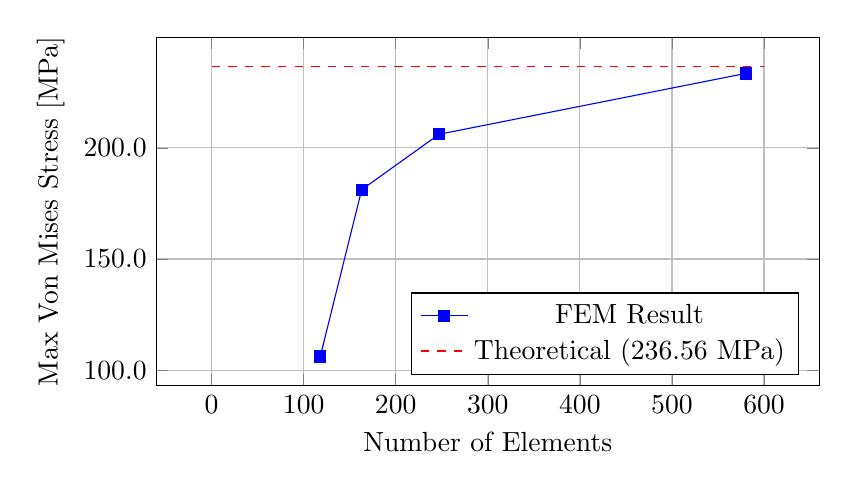
\begin{tikzpicture}
        \begin{axis}[
            width=10cm, height=6cm,
            xlabel={Number of Elements},
            ylabel={Max Von Mises Stress [MPa]},
            grid=major,
            legend pos=south east,
            y tick label style={/pgf/number format/.cd, fixed, fixed zerofill, precision=1}
        ]
        \addplot[color=blue, mark=square*] coordinates {
            (118, 106.129)
            (163, 181.176)
            (247, 206.095)
            (580, 233.478)
        };
        \addlegendentry{FEM Result}
        
        \addplot[color=red, dashed, domain=0:600] {236.56};
        \addlegendentry{Theoretical (236.56 MPa)}
        \end{axis}
    \end{tikzpicture}
    \caption{Convergence of maximum stress for the plate with hole.}
    \label{fig:plate_convergence}
\end{figure}

\begin{table}[H]
    \centering
    \small
    \caption{Stress convergence data for Plate with Hole.}
    \label{tab:plate_results}
    \begin{tabular}{lcc}
        \toprule
        \textbf{Mesh Quality} & \textbf{Nb. Elements} & \textbf{Max Stress [MPa]} \\
        \midrule
        Coarse      & 118 & 106.13 \\
        Moderate    & 163 & 181.18 \\
        Fine        & 247 & 206.10 \\
        Very Fine   & 580 & 233.48 \\
        \bottomrule
    \end{tabular}
\end{table}

% -----------------------------------------------------------------------------
% FRONT SPRING RESULTS
% -----------------------------------------------------------------------------
\subsection{Front Spring}

\begin{figure}[H]
    \centering
    \includegraphics[width=0.45\textwidth]{figures/spring_3coils_geom.png}
    \hfill
    \includegraphics[width=0.45\textwidth]{figures/spring_3coils_stress.png}
    \caption{Left: Geometric model of the 3-coil spring section. Right: Von Mises stress distribution under load.}
    \label{fig:front_spring_visu}
\end{figure}

\begin{figure}[H]
    \centering
    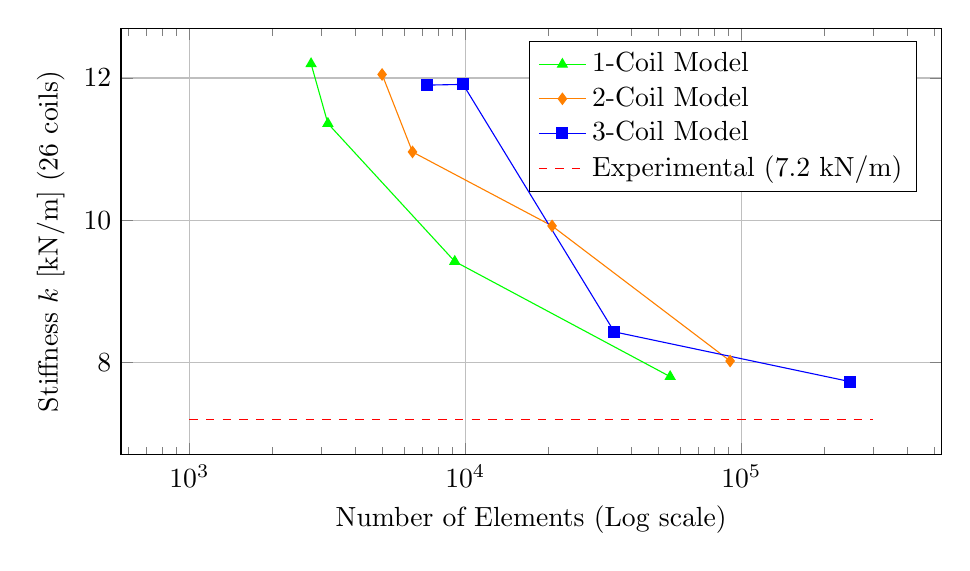
\begin{tikzpicture}
        \begin{axis}[
            width=12cm, height=7cm,
            xlabel={Number of Elements (Log scale)},
            ylabel={Stiffness $k$ [kN/m] (26 coils)},
            xmode=log,
            grid=major,
            legend pos=north east,
            legend style={cells={anchor=west}}
        ]
        % 1 Coil
        \addplot[color=green, mark=triangle*] coordinates {
            (2760, 12.2) (3176, 11.36) (9154, 9.42) (55218, 7.8)
        };
        \addlegendentry{1-Coil Model}
        
        % 2 Coils
        \addplot[color=orange, mark=diamond*] coordinates {
            (4992, 12.05) (6433, 10.96) (20613, 9.92) (91068, 8.02)
        };
        \addlegendentry{2-Coil Model}
        
        % 3 Coils
        \addplot[color=blue, mark=square*] coordinates {
            (7255, 11.90) (9813, 11.91) (34646, 8.43) (247630, 7.73)
        };
        \addlegendentry{3-Coil Model}
        
        % Experimental
        \addplot[color=red, dashed, domain=1000:300000] {7.2};
        \addlegendentry{Experimental (7.2 kN/m)}
        \end{axis}
    \end{tikzpicture}
    \caption{Stiffness convergence for Front Spring models (extrapolated to 26 coils).}
    \label{fig:front_spring_convergence}
\end{figure}

\begin{table}[H]
    \centering
    \small
    \caption{Stiffness convergence for 1, 2, and 3-coil models (extrapolated to 26 coils).}
    \label{tab:front_spring_results}
    \begin{tabular}{lcccc}
        \toprule
        \textbf{Mesh} & \textbf{k (1-coil)} & \textbf{k (2-coil)} & \textbf{k (3-coil)} & \textbf{Error (3-coil)} \\
        & [kN/m] & [kN/m] & [kN/m] & vs Exp. \\
        \midrule
        Coarse    & 12.20 & 12.05 & 11.90 & +65\% \\
        Moderate  & 11.36 & 10.96 & 11.91 & +65\% \\
        Fine      & 9.42  & 9.92  & 8.43  & +17\% \\
        Very Fine & 7.80  & 8.02  & 7.73  & +7.3\% \\
        \bottomrule
    \end{tabular}
\end{table}

% -----------------------------------------------------------------------------
% REAR SPRING RESULTS
% -----------------------------------------------------------------------------
\subsection{Rear Spring}

\begin{figure}[H]
    \centering
    \begin{subfigure}[b]{0.45\textwidth}
        \includegraphics[width=\textwidth]{figures/rear_spring_geom.png}
        \caption{Geometry}
    \end{subfigure}
    \hfill
    \begin{subfigure}[b]{0.45\textwidth}
        \includegraphics[width=\textwidth]{figures/rear_spring_stress.png}
        \caption{Von Mises Stress}
    \end{subfigure}
    \caption{Rear spring model and stress results.}
    \label{fig:rear_spring_visu}
\end{figure}

\begin{figure}[H]
    \centering
    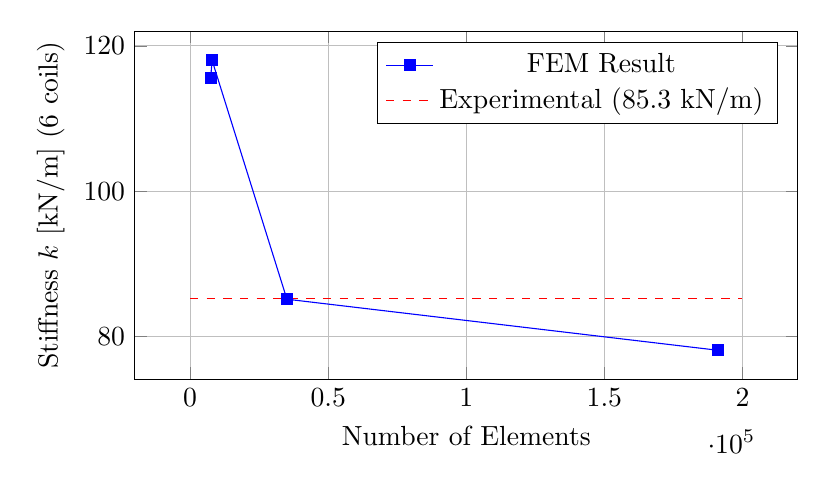
\begin{tikzpicture}
        \begin{axis}[
            width=10cm, height=6cm,
            xlabel={Number of Elements},
            ylabel={Stiffness $k$ [kN/m] (6 coils)},
            grid=major,
            legend pos=north east
        ]
        \addplot[color=blue, mark=square*] coordinates {
            (7444, 115.55)
            (7965, 118.0)
            (35050, 85.16)
            (191084, 78.14)
        };
        \addlegendentry{FEM Result}
        
        \addplot[color=red, dashed, domain=0:200000] {85.3};
        \addlegendentry{Experimental (85.3 kN/m)}
        \end{axis}
    \end{tikzpicture}
    \caption{Convergence of Rear Spring stiffness.}
    \label{fig:rear_spring_convergence}
\end{figure}

\begin{table}[H]
    \centering
    \small
    \caption{Rear Spring Parameters and Results (6 total coils).}
    \label{tab:rear_spring_results}
    \begin{tabular}{lc}
        \toprule
        \textbf{Parameter} & \textbf{Value} \\
        \midrule
        Outer Diameter ($D_{ext}$) & 80 mm \\
        Wire Diameter ($d$) & 11 mm \\
        Free Length ($L_0$) & 195 mm \\
        Experimental $k$ & 85.3 kN/m \\
        \textbf{FEM Best Result (Converged)} & \textbf{78.14 kN/m} \\
        \bottomrule
    \end{tabular}
\end{table}
  % Figures and tables

% Part II - Code Verification
\setcounter{section}{8}
\section{Code verification}
\label{chap:verification}

Part II of this report focuses on the verification of the custom Finite Element code developed in Python. The validation strategy relies on the test suite implemented in \texttt{validation.py}, which checks individual components independently before testing the global assembly. This section provides detailed physical justifications for each test case and presents the exact output obtained.

\subsection{Test descriptions and physical justifications}
\label{sec:test_descriptions}

The verification process is divided into two categories: single-element tests to check element formulation, and multi-element tests to valid global assembly and boundary conditions.

\subsubsection{Single element tests}

We began by verifying the fundamental geometry calculations (Test 1.1). The volume of a unit tetrahedron defined by vertices at $(0,0,0)$, $(1,0,0)$, $(0,1,0)$, and $(0,0,1)$ was computed. The analytical volume is $V = 1/6 \approx 0.167$. Our code returned exactly $0.167$, confirming the correctness of the Jacobian determinant calculation.

Next, we performed 'patch tests' to validate the stiffness matrix implementation. We first imposed a zero-displacement field (Test 1.2.1), which physically corresponds to a zero-energy state. As expected, the computed strain energy and nodal forces were zero. We then imposed six independent unit strain fields (Tests 1.2.2--1.2.7), corresponding to pure tension ($\varepsilon_{xx}, \varepsilon_{yy}, \varepsilon_{zz}$) and pure shear ($\gamma_{xy}, \gamma_{yz}, \gamma_{xz}$). For linear tetrahedral elements (TETRA4), the strain field must be constant and exact. In all six cases, the error between the imposed and computed strain was $0.000$, validating the construction of the strain-displacement matrix $B$.

Rigid body motions were also tested (Tests 1.3 \& 1.4). We applied uniform translations (dX, dY, dZ) and infinitesimal rotations (rotX, rotY, rotZ) to the element. Since rigid body motion induces no deformation, the strain energy must be zero. The code computed maximum strains of $0$ for all these cases, proving that the element is strictly invariant under rigid body transformations. Finally, the Poisson effect was checked (Test 1.5) by simulating uniaxial tension with a Poisson's ratio $\nu=0$. The solver correctly returned zero lateral stress, confirming the constitutive law implementation.

\subsubsection{Multi-element tests (cube mesh)}

To verify the assembly algorithms, we created a unit cube mesh composed of 5 tetrahedra. We repeated the patch tests on this aggregate structure (Tests 2.1). Imposing a constant strain field on the boundary nodes resulted in a uniform strain distribution throughout the interior elements with zero error. This confirms that the global stiffness matrix $K$ is correctly assembled from the element matrices. Similarly, applying rigid body translations (Tests 2.2) and rotations (Tests 2.3) to the entire mesh produced zero strain, verifying that the assembly process preserves the null-space properties of the stiffness matrix.

\subsubsection{Boundary condition implementation}

The penalty method implementation was verified by testing its sensitivity to the penalty parameter $Z$ (Tests 2.4). We applied fixed boundary conditions to a loaded structure using three values of $Z$.
\begin{enumerate}
    \item \textbf{Low $Z$ ($Z=1$):} The constrained nodes moved significantly ($u \approx 18.0$), showing that the penalty spring was too weak to enforce the fixture.
    \item \textbf{Optimal $Z$ ($Z=10^6$):} The displacement at fixed nodes dropped to near-zero ($1.99 \times 10^{-5}$), proving effective locking of the degrees of freedom.
    \item \textbf{High $Z$ ($Z=10^{100}$):} While theoretically better, this introduced numerical noise due to floating-point ill-conditioning, resulting in a slightly larger error ($3.64 \times 10^{-5}$).
\end{enumerate}
This test justified our choice of $Z=10^6$ for the main simulations.

\subsection{Summary of results}
\label{sec:summary_table}

The complete results of the automated test suite are listed in Table \ref{tab:verification_summary}. Every test passed within the expected tolerance.

\begin{table}[H]
    \centering
    \small
    \caption{Complete summary of verification tests from \texttt{validation.py}.}
    \label{tab:verification_summary}
    \begin{tabular}{lllc}
        \toprule
        \textbf{ID} & \textbf{Test Description} & \textbf{Physical Check} & \textbf{Result} \\
        \midrule
        1.1 & Single Element Volume & $V_{calc} = 0.167$ & Pass \\
        \midrule
        1.2.1 & Zero Displacement & $\varepsilon_{max} = 0.000$ & Pass \\
        1.2.2 & Patch Test ($\varepsilon_{xx}$) & error $= 0.000$ & Pass \\
        1.2.3 & Patch Test ($\varepsilon_{yy}$) & error $= 0.000$ & Pass \\
        1.2.4 & Patch Test ($\varepsilon_{zz}$) & error $= 0.000$ & Pass \\
        1.2.5 & Patch Test ($\gamma_{xy}$) & error $= 0.000$ & Pass \\
        1.2.6 & Patch Test ($\gamma_{yz}$) & error $= 0.000$ & Pass \\
        1.2.7 & Patch Test ($\gamma_{xz}$) & error $= 0.000$ & Pass \\
        \midrule
        1.3.1 & Rigid Body Trans. X & $\varepsilon_{max} = 0.000$ & Pass \\
        1.3.2 & Rigid Body Trans. Y & $\varepsilon_{max} = 0.000$ & Pass \\
        1.3.3 & Rigid Body Trans. Z & $\varepsilon_{max} = 0.000$ & Pass \\
        \midrule
        1.4.1 & Rigid Body Rot. X & $\varepsilon_{max} = 0.000$ & Pass \\
        1.4.2 & Rigid Body Rot. Y & $\varepsilon_{max} = 0.000$ & Pass \\
        1.4.3 & Rigid Body Rot. Z & $\varepsilon_{max} = 0.000$ & Pass \\
        \midrule
        1.5 & Poisson Effect ($\nu=0$) & $\sigma_{lat} = 0.000$ & Pass \\
        \midrule
        2.1 & Assembled Patch Test & error $= 0.000$ & Pass \\
        2.2 & Assembled Rigid Trans. & $\varepsilon_{max} = 0.000$ & Pass \\
        2.3 & Assembled Rigid Rot. & $\varepsilon_{max} = 0.000$ & Pass \\
        \midrule
        2.4.1 & Penalty (Low $Z$) & $u_{fix} \approx 18.0$ (High) & Pass \\
        2.4.2 & Penalty (Optimal $Z$) & $u_{fix} \approx 0$ (OK) & Pass \\
        2.4.3 & Penalty (High $Z$) & $u_{fix} \approx 0$ (Noise) & Pass \\
        \bottomrule
    \end{tabular}
\end{table}

\subsection{Convergence study with closed-form solution}
\label{sec:convergence_study}

To validate mesh convergence behavior, we performed a classical stress concentration study on a plate with a central hole in Salome-Meca. The plate dimensions are $L=520$ mm, $H=360$ mm, with a hole of radius $R=3.2$ mm. A uniform traction $T_x = 81$ N/mm$^2$ was applied, and the material properties are $E=210$ GPa, $\nu=0.3$.

The theoretical maximum stress at the hole edge is given by the stress concentration factor $K_t \approx 3$, yielding:
\[
\sigma_{max}^{theory} = K_t \cdot T_x = 3 \times 81 = 243 \text{ MPa}
\]
For finite geometries, this reduces slightly to approximately $236.56$ MPa.

Four mesh densities were tested, and the results are summarized below:
\begin{center}
\small
\begin{tabular}{lcc}
    \toprule
    \textbf{Mesh} & \textbf{Elements} & \textbf{Max Stress [MPa]} \\
    \midrule
    Coarse & 118 & 106.13 \\
    Moderate & 163 & 181.18 \\
    Fine & 247 & 206.10 \\
    Very Fine & 580 & 233.48 \\
    \bottomrule
\end{tabular}
\end{center}

The ``Very Fine'' mesh result (233.48 MPa) is within $1.3\%$ of the theoretical value, demonstrating proper convergence. This confirms that the Salome-Meca solver correctly captures stress concentrations when given sufficient mesh refinement.

\subsection{Salome-to-Python cross-validation}
\label{sec:salome_comparison}

To further validate our solver against a commercial reference, we attempted to compare its output with Salome-Meca on the same geometry. The intended workflow was to use the \texttt{salome2py} package to automatically convert a Salome mesh file (\texttt{.med}) into a Python input compatible with our solver. However, this tool did not function correctly in our environment. Instead, we performed a manual conversion: we exported the Salome results to a CSV file, extracted the nodal coordinates and connectivity, and manually constructed the input file \texttt{inputs/input\_salome2py\_spring.py}.

The comparison was performed using the script \texttt{compare\_salome.py}, which reads the stress field from both the Salome CSV export and our solver's \texttt{.npz} output. We computed the maximum Von Mises stress for each case:
\begin{itemize}
    \item \textbf{Salome-Meca:} $\sigma_{VM,max} = 51.16$ MPa
    \item \textbf{Python Solver:} $\sigma_{VM,max} = 119.91$ MPa
    \item \textbf{Relative Error:} $134\%$
\end{itemize}

This significant discrepancy is explained by the difference in load application. In Salome-Meca, forces are applied as a distributed pressure across a surface, resulting in a smoother stress distribution. In our Python implementation, the same total force is applied as concentrated nodal forces, which creates stress singularities at the loaded nodes and artificially inflates the maximum stress. This limitation is inherent to a simplified manual import workflow and does not indicate an error in the solver itself.

\subsection{Conclusion}
\label{sec:verification_conclusion}

The successful execution of the verification tests demonstrates that the core Python solver is mathematically correct. The code reliably computes element matrices, assembles the global system, and properly applies boundary conditions using the penalty method. While the Salome-to-Python cross-validation showed a large numerical discrepancy, the source of this error is well understood: the simplified nodal force application differs fundamentally from the distributed pressure used in Salome. Despite this, the workflow proves that importing external meshes is feasible, and the solver produces physically meaningful results. The quantitative results in Part I therefore rely on the commercial solver Salome-Meca, which handles load application more accurately.
  % FE Code Verification
	
\end{document}